\chapter[B-arbres]{Cas concret : B-arbres%
\chaptermark{B-arbres}}
\section{Définitions}
Un B-arbre est une structure de données en arbre équilibré. Le principe général de cette structure est la minimisation de la taille des arbres en permettant aux noeuds la possession de plusieurs clés. Un B-arbre est donc caractérisé par les propriétés suivantes :
\begin{itemize}
\item Un ordre $m$
\item Chaque noeud contient $k$ clés triées avec :
\begin{itemize}
\item pour le noeud racine : $m \leq k \leq 2m$
\item pour un noeud non racine : $1 \leq k \leq 2m$
\end{itemize}
\item Un noeud est soit :
\begin{itemize}
\item Terminal et donc est une feuille.
\item Non terminal et possède alors $k+1$ fils. Les clés du $i$\up{ème} fils ont des valeurs comprises entre les valeurs des $(i-1)$\up{ème} et $i$\up{ème} clés du père.
\end{itemize}
\item Chaque chemin de la racine à une feuille est de même longueur $h$ (hauteur).
\end{itemize}

\begin{figure}[h]
	\centering
	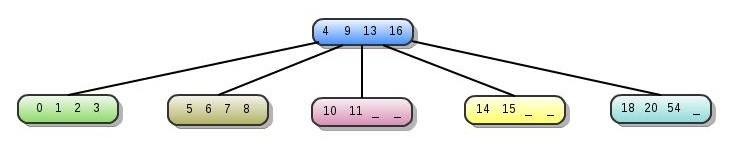
\includegraphics[scale=0.5]{barbre}
	\caption{Exemple de B-arbre}
	\label{fig:barbre}
\end{figure}

Étant donné la forme dont sont stockées les données dans les B-arbres (tri) et l'exécution des opérations d'insertion et de suppression en temps amorti logarithmique, cette structure est principalement mise en œuvre dans les mécanismes de gestion des bases de données et des systèmes de fichiers.
\section{Implémentations}
\subsection{Méthodologie et choix de structure}
En considérant les propriétés des B-arbres décrites précédemment, nous avons procédé dans la construction de nos structures/algorithmes de la manière suivante : 
\begin{enumerate}
\item Mise en place de classes génériques en utilisant le principe des “templates”: L’objectif de cette approche est de générer le code spécifique à chaque type à partir d'un modèle générique. L’intérêt de cette technique est double : nous disposons d’un code optimisé pour chaque type et le code source n'est pas dupliqué car il écrit un méta-code à partir duquel sont générés les codes spécifiques. Nous avons donc paramétré nos arbres par le type de données à stocker et nous avons choisi de fixer l’ordre du B-Arbre.
\begin{lstlisting}
//T un type quelconque et k l ordre de l arbre
template<class T,short k>
\end{lstlisting}
\item     Mise en place de la structure de noeud "\verb+BTreeItem+": Cette structure comporte les éléments suivants :
\begin{itemize}
\item     Deux variables \verb+k+ et \verb+nCount+ de types entier court représentant respectivement l'ordre de l'arbre et le nombre de clés stockés dans un noeud.
\item     Un tableau \verb+data+ de $2 \times k$ clés rangées dans l'ordre croissant.
\item     Un tableau \verb+subItems+ de $2\times k+1$ pointeurs vers les enfants du noeud lorsque celui-ci n'est pas une feuille.
\end{itemize}
Cette structure possède également deux fonctions qui nous serviront dans la méthode d’insertion dans le B-arbre :
\begin{itemize}
\item     Une fonction de recherche dichotomique\cite{dichotomie} \verb+searchInNode+.
\item         Une fonction de "découpage" de noeud \verb+SplitNode+.   
\end{itemize}
\item     Mise en place de la structure d’arbre complète \verb+BTree+ : cette structure comporte les fonctions nécessaires pour la recherche d’un élément dans l’arbre, la suppression ainsi que l’ajout. Nous verrons ces fonctionnalités plus en détails dans les parties qui suivent.
\end{enumerate}

\subsection{Méthode de recherche}
La recherche est effectuée de la même manière que dans un arbre binaire de recherche, d'où l'utilisation de la fonction de recherche dichotomique citée précedemment. Partant de la racine, nous parcourons récursivement l’arbre. À chaque nœud, nous choisissons le sous-arbre fils dont les clés sont comprises entre les mêmes bornes que celles de la clé recherchée.
\paragraph{Algorithme} Nous avons la structure de noeud suivante :
\begin{figure}[hbt]
	\centering
	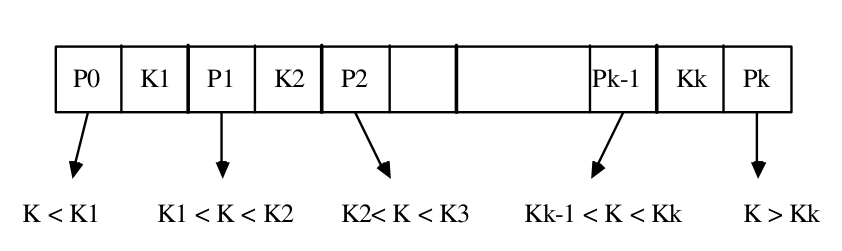
\includegraphics[scale=0.5]{node}
	\caption{Représentation de la structure}
	\label{fig:node}
\end{figure}

avec $K_1 < K_2 < K_3 < \dots < K_n$ clés et $P_0$,...,$P_k$ pointeurs vers noeuds enfants.

Pour chercher une clé $k$ dans le B-arbre, l'algorithme récursif a été imaginé à partir des grandes étapes suivantes : 

A partir de la racine et pour chaque noeud, on examine :
\begin{itemize}
\item {si la clé est présente}    succès
\item {si K<K1} recherche dans P_0
\item {si K>Kn} recherche dans P_k
\end{itemize}

